\documentclass[a4paper,11pt]{article}
\usepackage[spanish]{babel}
\usepackage[utf8]{inputenc}
\usepackage{hyperref}
\usepackage[left=2cm, right=2cm, top=2cm]{geometry}
\usepackage[pdftex]{graphicx}


\begin{document}

\title{RNA no codificante en cáncer}
\author{Álvaro Andrades Delgado}
\date{\today}
\maketitle

\begin{abstract}

En el presente texto, se recoge una revisión sobre el papel de los RNAs no codificantes en cáncer. Se comienza con una breve historia sobre los principales hallazgos acerca de las funciones biológicas de los RNAs no codificantes, para pasar a continuación a resumir el estado del arte. URL del repositorio en GitHub: \url{https://github.com/alvaro-andrades/proyecto_final} 

\textbf{Palabras clave:} RNA no codificante, microRNA, RNA largo no codificante.

\end{abstract}



\section{Introducción}

Según la visión clásica del dogma central de la biología molecular, el DNA de las células se transcribe a RNA, el cual a su vez se traduce a proteínas\cite{Kung2013}. Según esta visión clásica, el RNA actúa como un mero intermediario entre el DNA y las proteínas. Así, clásicamente se identificaron tres tipos principales de RNA: el RNA mensajero (mRNA), el RNA de transferencia (tRNA) y el RNA ribosómico (rRNA)\cite{Cech2014}.

La visión clásica sobre el papel del RNA en la célula comenzó a cambiar en las últimas décadas del siglo XX, cuando comenzaron a descubrirse RNAs que no correspondían a ninguno de los tres tipos clásicos de RNA\cite{Cech2014}. Además, comenzaron a publicarse estudios que apuntaban a la existencia de RNAs con actividad catalítica, la cual únicamente se atribuía a proteínas\cite{Kruger1982}, así como al papel de RNAs no codificantes de proteína en la regulación de la expresión génica\cite{Brannan1990}. Sin embargo, no fue hasta los estudios realizados en \textit{C. elegans} a inicios de la década de los 2000 cuando comenzó a aceptarse en la comunidad científica que los RNAs no codificantes de proteína pueden desempeñar funciones relevantes biológicamente\cite{Grishok2001}. Hoy en día, se conoce una lista extensa de tipos de RNAs, la cual va mucho más allá de las funciones \verb="clásicas"= del RNA (Tabla \ref{table:ncRNAs}).


\section{Estado del arte}

En la última década, se han producido grandes avances en el conocimiento sobre el papel de RNAs no codificantes en cáncer. Un ejemplo es el de los RNAs largos no codificantes (lncRNAs), de los cuales se sabe a día de hoy que se encuentran implicados en todas las funciones características de las células tumorales\cite{Schmitt2016}(Figura \ref{fig:hallmarks}).

Otros RNAs no codificantes ampliamente estudiados en la actualidad son los microRNAs (miRNAs). Los miRNAs participan en la regulación de la expresión génica y, en consecuencia, a menudo se encuentran alterados en cáncer\cite{Medina2008}.

En la actualidad, hay un gran interés por investigar las alteraciones que sufren los RNAs no codificantes en cáncer, hasta el punto de que se han creado grandes consorcios para secuenciar genomas completos de pacientes de cáncer y, así, determinar las alteraciones que presentan en genes no codificantes\cite{Khurana2016}.
\newpage


\section{Imágenes y tablas}

\begin{table}[h!]
\begin{tabular}{p{2cm}p{5cm}p{9cm}}
\textbf{Abreviación} & \textbf{Nombre} & \textbf{Descripción} \\
\hline
lncRNA & RNA largo no codificante & RNA que no codifica proteína y presenta una longitud superior a 200 nucleótidos. \\
miRNA & microRNA & RNA no codificante con una longitud de 18-22 nucleótidos y que participa en el silenciamiento de la expresión génica mediante la unión específica a mRNAs diana. \\
mRNA & RNA mensajero & RNA cuya secuencia contiene las instrucciones para sintetizar una proteína. \\
piRNA & RNA asociado a PIWI & RNA que participa en la modificación de la cromatina para reprimir la transcripción génica. \\
rRNA & RNA ribosómico & RNA componente de los ribosomas. Presenta función estructural y catalítica. \\
snoRNA & RNA nucleolar pequeño & RNA que participa en la biogénesis del rRNA. \\
snRNA & RNA nuclear pequeño & RNA localizado en el núcleo de células eucariotas. \\
\hline
\end{tabular}
\caption{Lista de los principales tipos de RNAs no codificantes identificados en la actualidad. Adaptado de \cite{Cech2014}.}
\label{table:ncRNAs}
\end{table}


\begin{figure}[h!]
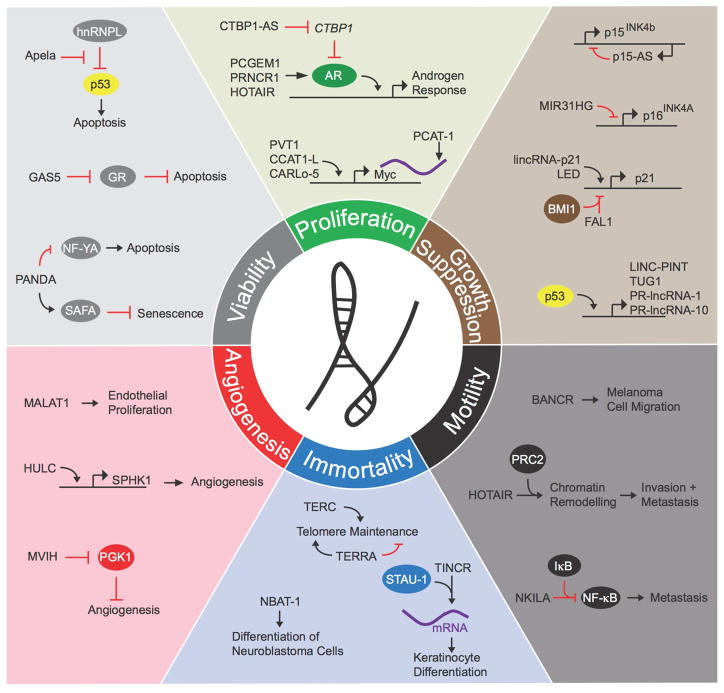
\includegraphics{figuras/hallmarks.jpg}
\caption{Implicación de los RNAs largos no codificantes (lncRNAs) en las principales características distintivas del cáncer. Figura tomada de \cite{Schmitt2016}.}
\label{fig:hallmarks}
\end{figure}


\section{Fórmulas}

Dado que no existen fórmulas relevantes en el estudio de la biología molecular de los RNAs no codificantes, a continuación se incluye la fórmula de la ecuación de Dirac:\\
$(\beta m c^2 + c (\sum_{n=1}^3\alpha_n p_n)) \psi(x,t) = i\hbar \frac{\partial \psi(x,t)}{\partial t}$\\


\bibliography{bibliografia}
\bibliographystyle{plain}



\end{document}
